

\chapter{预等离子体对于加速的增强作用}
\label{chap:preplasmaEhancement}

\section{预脉冲与预等离子体}
\begin{figure}[!htbp]
  \centering
  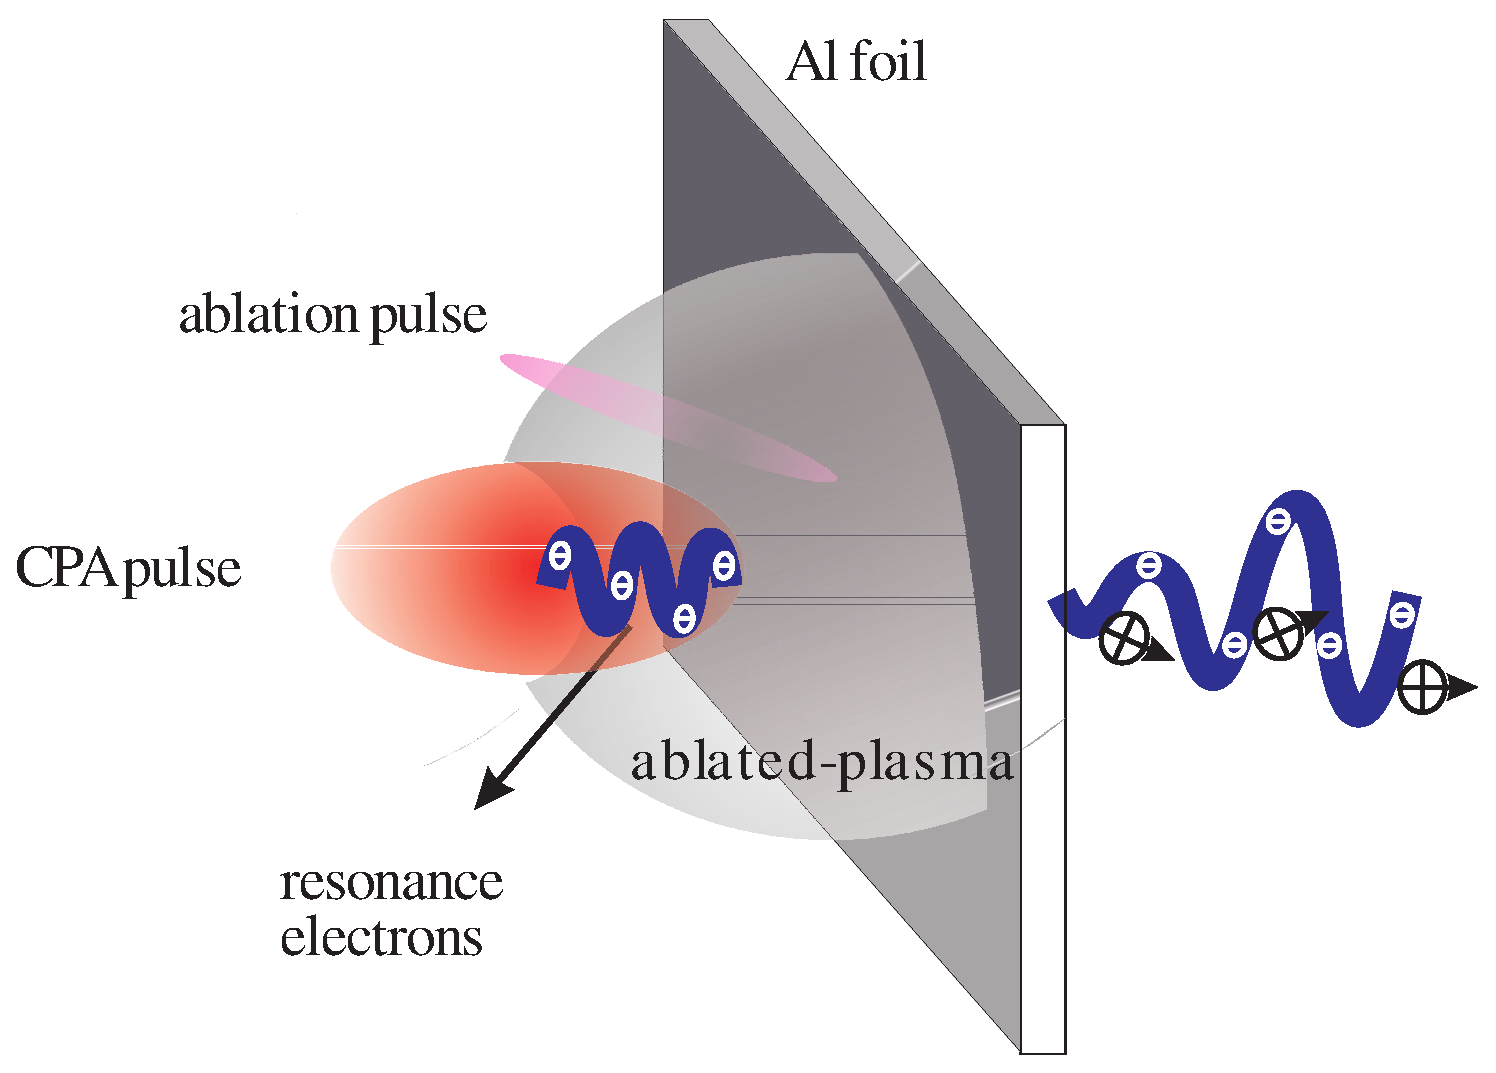
\includegraphics[width=\MyFactor\textwidth]{Img/enhancement.eps}
  \caption{预脉冲增强作用示意图}
  \label{fig:prepulse2012}
\end{figure}



上一章中,我们利用激光的预脉冲或者中等强度激光脉冲($10^{10}W/cm^2$ 到 $10^{14}W/cm^2$),对于金属靶进行烧蚀,产生预等离子体。预等离子体由靶前表面向外传播,其密度一维分布为类指数函数,其中一部分处于临界密度领域。我们已经对于临界密度做出定义,与激光频率一致的等离子体波对应的密度,同时也是非相对论激光脉冲穿透密度极限。而当激光的光强到达相对论区域,等离子体频率由于相对论效应相应地降低,因此激光穿透等离子体的能力增强,而此时等离子体也称为临界密度等离子体。

\begin{figure}[!htbp]
  \centering
  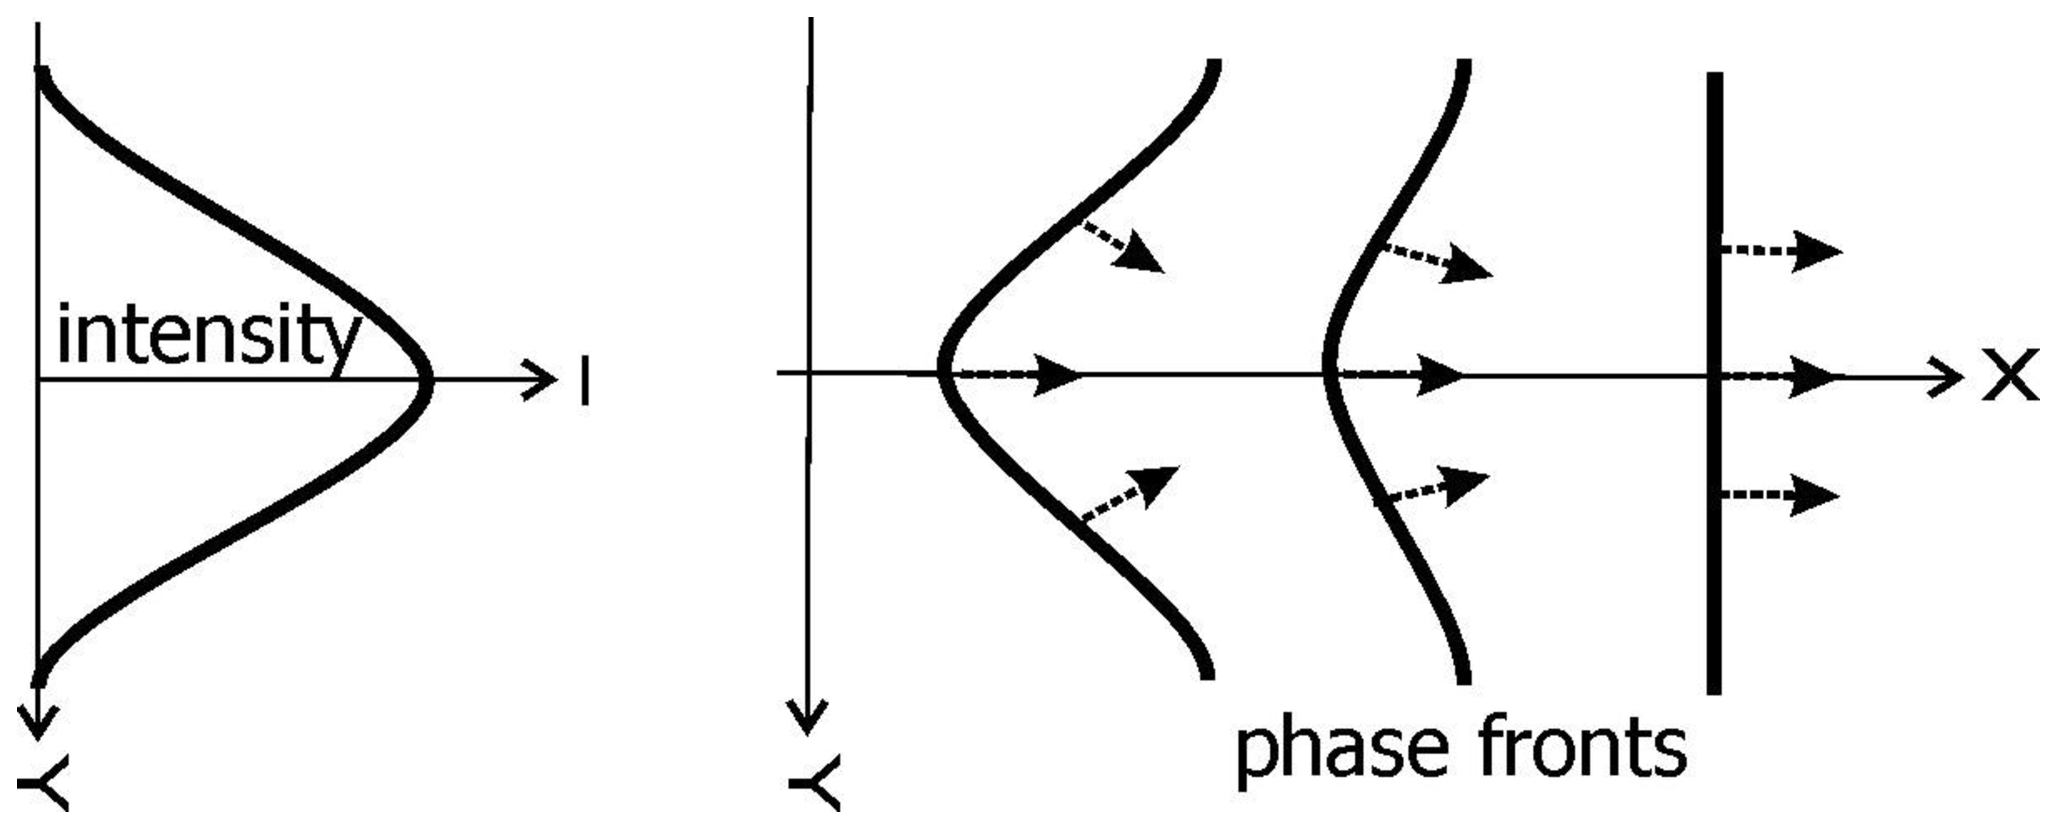
\includegraphics[width=\MyFactor\textwidth]{Img/selffocussing.eps}
  \caption{激光自聚焦示意图}
  \label{fig:selffousing}
\end{figure}

\begin{figure}[!htbp]
  \centering
  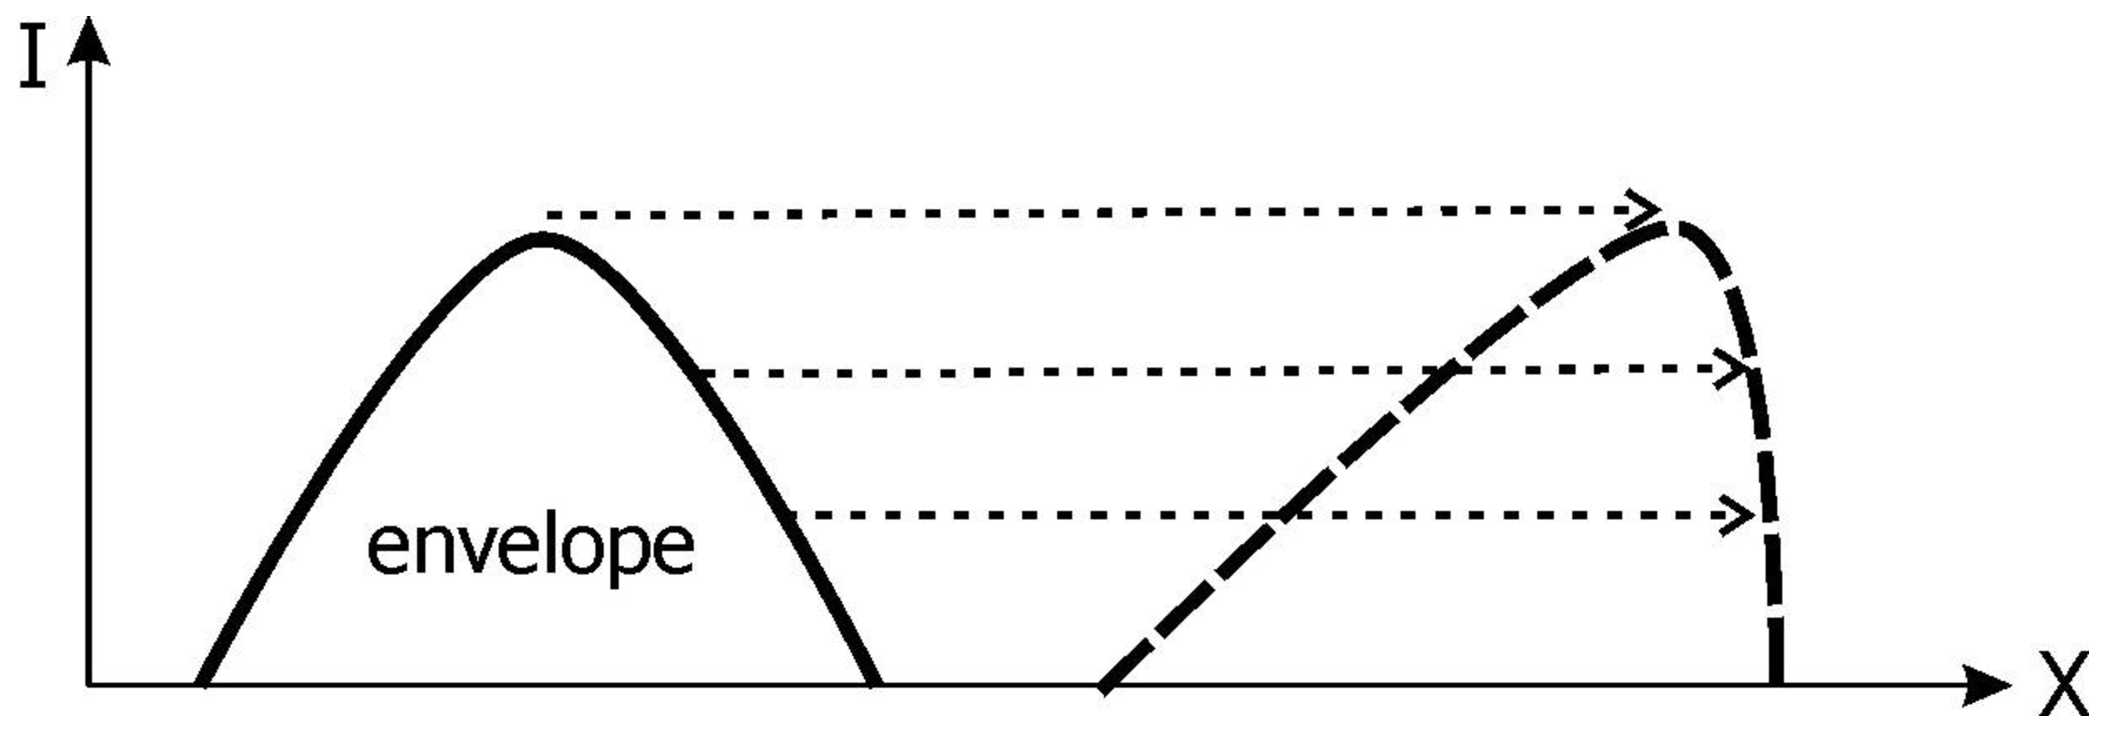
\includegraphics[width=\MyFactor\textwidth]{Img/prof-steepening.eps}
  \caption{激光自相位调制}
  \label{fig:phaseModulate}
\end{figure}




在激光在等离子体传播的过程中,存在很多的非线性机制。由于激光脉冲横纵向分布,对于等离子体折射率的调制,会产生相对论自聚焦以及相对论相位自调制现象。相对论自聚焦,是由于纵向高斯分布激光使得折射率中间低两翼高,像棱镜般对于激光脉冲形成聚焦效果,横向尺寸变小。另一方面,纵向高斯分布使得激光波前群速度较低,发生相对论相位自调制,使得激光脉冲纵向压缩。最终,由于相对论自聚焦以及自调制作用,激光的峰值光强得到明显的提高,横纵向尺寸得到有效的压缩\cite{wang2011laser}。
与此同时,激光脉冲前沿的电子被激光有质动力排开,形成横向尺寸与激光焦斑大小相当的离子通道结构。通道中电子密度中间低,通道壁较高,且一部分电子在通道壁回流产生磁场。然而离子分布均匀,电子与离子在通道中静电分离,通道中形成了的静电势,通道中的电子  在静电势中作betatron震荡。此外,这些betatron共振电子受到激光场的驱动作用,当betatron震荡频率与激光频率匹配时,共振现象发生,使得电子产生强烈的能量吸收,这种现象被称为DLA(Direct Laser Acceleration)。共振电子的横向震荡频率即激光频率$\omega_0$,纵向的频率由于  是$2 \omega_0$。共振电子产生之后沿激光方法传播,同时由于通道壁电子回流产生的磁场聚焦作用,形成高能量密度的束流。关于DLA的系统研究属于A. Pukhov和J. Meyer-ter-Vehn以及盛正明\cite{pukhov1998relativistic,pukhov1999particle},通过模拟和实验,得出电子的温度的定标率,
\begin{equation}
\label{eqn:DLAtemperature}
T_e = 1.8(I_{cpa} {\lambda}^2/{13.7}GW)^{1/2}
\end{equation} 

相对于同等光强的相对论有质动力加热,其温度有三倍以上的提高,且电子的能量密度较高,于是将共振电子用于质子加速能够有效。

\begin{figure}[!htbp]
  \centering
  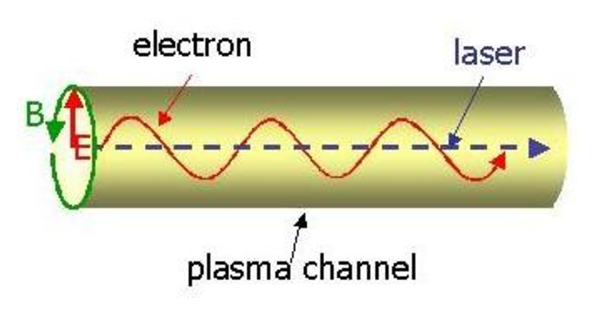
\includegraphics[width=\MyFactor\textwidth]{Img/IFEL.eps}
  \caption{逆自由电子激光示意图}
  \label{fig:IFEL}
\end{figure}


在我们的加速方案中,使用激光预脉冲产生预等离子体,激光主脉冲与预脉冲作用产生DLA共振电子。激光能量有效地转化给电子,而后电子传播至靶后形成鞘层场加速离子,最终对于离子加速产生增强的作用。整个加速方案的模型,首先强度$10^{12}W/cm^2$,脉冲时间$100ps$量级烧蚀脉冲与$\mu m$量级的金属靶作用。通过调整烧蚀脉冲的强度以及持续时间,控制金属靶的烧蚀深度和预等离子体膨胀距离以及密度梯度,最终得到指数密度分布预等离子体与未烧蚀金属靶的双层靶结构。而后相对论强度的激光与双层靶作用,首先激光脉冲在预等离子体临界密度区域中产生高能量高密度的DLA共振加热电子,共振电子传输到靶后面,在靶后建立起鞘层静电加速场。未烧蚀的金属靶的作用,提供质子层并提供未破坏的后表面。在这一模型的基础上,我们对于加速有如下的理论估计:
首先,加速的过程是在后表面由于电子产生的鞘层加速场产生的,仍然归类为TNSA加速机制。
相对于有质动力加热,其电子温度大约三倍,且其能量密度较高。
对于加速时间,我们采用fuchs的 $1.3 t_{laser}$的估计。 利用TNSA理论中,估计质子的能量增加至少三倍,而电子的温度是重要原因。


问题的关键在于如何确保电子的温度可以达到最大值,而且保证高能量高密度的电子可以传播达到靶的后面。DLA电子高能高密,是由于共振效应,以及通道中磁场的聚焦效果的作用。因此电子能量密度,重要的条件是通道的存在,使得电子达到固体靶之前(因为固体靶中的电子由于相互之间的空间电荷力产生的密度减小可以忽略)仍然保持高度的聚焦状态。因此最优的加速条件:
激光在即将达到固体靶的时候耗尽所有的能量,即DLA共振电子获得最大程度的能量增益的同时,确保激光脉冲产生的通道能够一直连接到金属靶,有助于电子保持聚焦的高密度状态。
电子的加热和传输在很大程度上决定于等离子体的密度,而预等离子体的分布由预脉冲决定,因此可以通过控制预脉冲的参数,满足最优条件。对此我们有如下的估计:

1激光的焦斑半径$r_0$与通道半径相当
2激光能量有到共振电子的比例为$\alpha$, 于是共振电子能量$E_{e} =\alpha E_{laser} $,且$E_{laser}=\pi {w_0}^2 I_{cpa} \tau_{cpa}$
3当共振电子的温度最高时,其能量可估计为:

\begin{equation}
\label{eqn:energyOsilationElectron}
 \pi {w_0}^2 {{\int}_{0}}^{x_{front}} density(x) \times T_e
\end{equation}

其中 $x_{front}=c_s {\tau}_{abl}[2ln({\tau}_{abl} {\omega}_{pi})+ln2-3]$\cite{mora2003plasma}    是预等离子体膨胀前沿,预等离子体密度分布$density(x)=n_c exp(-x/{c_s{\tau}_{abl}})$, ${\omega}_{pi}$是热电子对应等离子体频率, ${\tau}_{abl}$是烧蚀脉冲时间尺寸,烧蚀脉冲强度$I_{abl}$ 包括在离子声速$c_s$中。考虑条件2,得到



\begin{equation*}
\label{eqn:OptimalCondition}

{1.8} c_s {\tau}_{abl}[1-exp(-x_{front}/{c_s{\tau}_{abl}})] 
 = {\alpha}_{absorb} a_{cpa} \tau_{cpa}.

\end{equation*}








在此基础上我们做了模拟仿真的研究,二维PIC粒子仿真,使用KLAP代码,基本情况如下:
其中的参数是依据北京大学强激光实验室的实验条件,金属靶材质是密度为2.7$g/cm^3$铝靶,厚度为$\mu m$量级。 激光参数包括有:预脉冲以及主脉冲。预脉冲的强度: $10^12W/cm^2$,且预脉冲的时间尺度为1ns之内。主激光脉冲在预脉冲之后,强度$10^20W/cm^2$,聚焦后的焦斑半径为5$\mu m$,激光的脉冲持续时间为$30fs$,对应的脉冲能量为5J。   经过烧蚀之后的靶的分布由MULTI计算的结果导入,其结构为双层靶,10$\mu  m$量级的预等离子体与$\mu m$厚度的金属靶。 PIC模拟中的参数如下:仿真区域$80 \times 40 \mu m^2$,格点数目$6400 \times 3200$, 其分辨率为$\lambda / 8$。仿真时间为200T, T为激光周期,对应于$3.3fs$。 激光脉冲在50T进入仿真区域,在100T达到金属靶的位置,$t=200T$时加速过程已经完全结束了。在此基础上,我们改变了预脉冲的持续时间,得到不同的预等离子体分布,并保持其他的条件不变,做了令两组仿真。

对于仿真的结果我们的分析如下:
首先是激光在预等离子体中传播并将能量传递给共振电子的过程。如图所示(\ref{fig:laserEvolution}),在其中\ref{fig:laserEvolution}(a) 是激光聚焦的过程,$t=50T$的时候激光开始进入预等离子体,并在其中传播。之后$t=80$脉冲进入强聚焦的过程,激光的强度的增加剧烈,并且伴随着成丝等不稳定性的出现。$t=100T$激光波前达到金属靶的位置,其能量基本耗散。整个过程中,激光的能量很少有反射的成分,伴随着聚焦过程的增强,共振电子产生。在\ref{fig:laserEvolution}(b),电子的能量密度分布。 其中心位置处的电子呈现出明显的周期性结果,且其周期为激光的周期,而不是由于所谓的有质动力加速所产生的二倍于激光频率的结构。而且在现有的机制中,且其能量密度比有质动力加速有着明显的提高。在$t=100T$的时候,紧聚焦的电子束流达到靶后,形成鞘层的同时,由于没有磁场约束力的作用,迅速的散开。在\ref{fig:laserEvolution}(c)中,离子通道很明显的连接到了固体靶位,将共振电子传输到了靶后。










对比试验的结果在 \ref{fig:laserEvo} 中,对比以上模拟,左侧的模拟中,预脉冲的持续时间为100ps,而右侧的预脉冲持续时间为280ps。直接的结果就是预等离子体的分布的变化,其中100ps对应的膨胀距离较小,而且等离子体的密度中梯度较大。而280ps对应的等离子体的膨胀距离较大,而且密度梯度较小。同样做了激光脉冲聚焦在\ref{fig:laserEvolution}(a)中, 很明显, 左侧的激光在没有达到最优聚焦的时候已经被反射了,而右侧的激光脉冲在没有达到固体靶的时候已经完全的耗散。对应于共振电子的产生的情况在\ref{fig:laserEvolution}(b),其中左侧的电子的能量密度较低原因在于激光能量未能完全的转化,右侧的电子能量密度在 激光聚焦区域很高,但是由于激光在耗散之后,没有相应的通道提供聚焦磁场,因此很快就散开。\ref{fig:laserEvolution}(c)中给出了通道的形成,可以很明显的得到结论,当预等离子体的尺寸过长时,激光脉冲无法完全穿透,从而无法实现通道连接到固体靶。 为了跟好地理解等离子体中的电子的加热的情况,我们统计了预等离子体中的电子加热的情况以及固体靶中的电子加热的情况。ref{fig:laserEvolution}(g)为预等离子体中的电子加热的情况,其中红,黑,蓝分别代表着‘最优’,‘较短’,‘较长’的等离子体分布。‘最优’和‘较长’的预等离子体中的电子加热情况类似,可见都已经达到了共振电子加热的极限的情况,而‘较短’中的电子加热由于激光的吸收不完全,能量较低。在ref{fig:laserEvolution}(h),统计了固体靶中的电子的能谱,‘最优’,‘较长’情况中由于激光在达到靶的时候已经基本耗散,所有没有太多的能量沉积在固体靶子中,而对于‘较短’,电子的加热很明显,由于激光脉冲在固体靶表面有很强烈的反射,因此加热存在。考虑加热电子的总的温度以及相应的树木,‘较长’,‘最优’相对于‘较短’有着明显的优势,但是由于‘较长’情况下,通道终止于激光消失处,因此无法进一步的进行共振电子的聚焦,造成了ref{fig:laserEvolution}(d)所示的束流散开的情况,对于最终的加速有一定的影响。




根据以上的结果,我们根据mora的自由膨胀的模型进行验证,因为电子的问题已经给出,而且电子的密度可以从模拟中得到相应的值,加速的时间可以从fochs的估计中得到,因此加速的能量应该在90MeV。 我们对此作用质子的能谱,且把三种情况和没有预等离子体膨胀的情况进行了相应的对比,得到的结果在\ref{fig:preplasmaCompare}(h)






与此同时我们开始,寻找不同的预脉冲与主脉冲的匹配关系。由于我们的研究表明在,在固定预脉冲与主脉冲的强度的前提下,预脉冲的持续时间应该是和主脉冲的持续时间存在一定的正比关系

